% !TEX root = ../../main.tex

\subsection{Thermal stability}

In order to check if the shaped samples have not undergone bulk
structural changes

The process of shaping did not have any impact on the thermal stability of 
the investigated MOFs, as evidenced by the TGA curves 
(Figure~\ref{fig:shaping:tgacurves}). The primary mass loss occurs 
in a \SI{10}{\degreeCelsius} range for all powder-pellet pairs.
Shaped samples are expected to have a smaller percentage mass loss 
overall due to the addition of the temperature inert alumina.

\begin{figure}
    \centering
    
    \begin{subfigure}{0.6\textwidth}
        \parbox[c]{0.1\linewidth}{\caption{}\label{fig:shaping:tgauio66}}%
        \parbox[b]{0.7\linewidth}{%
        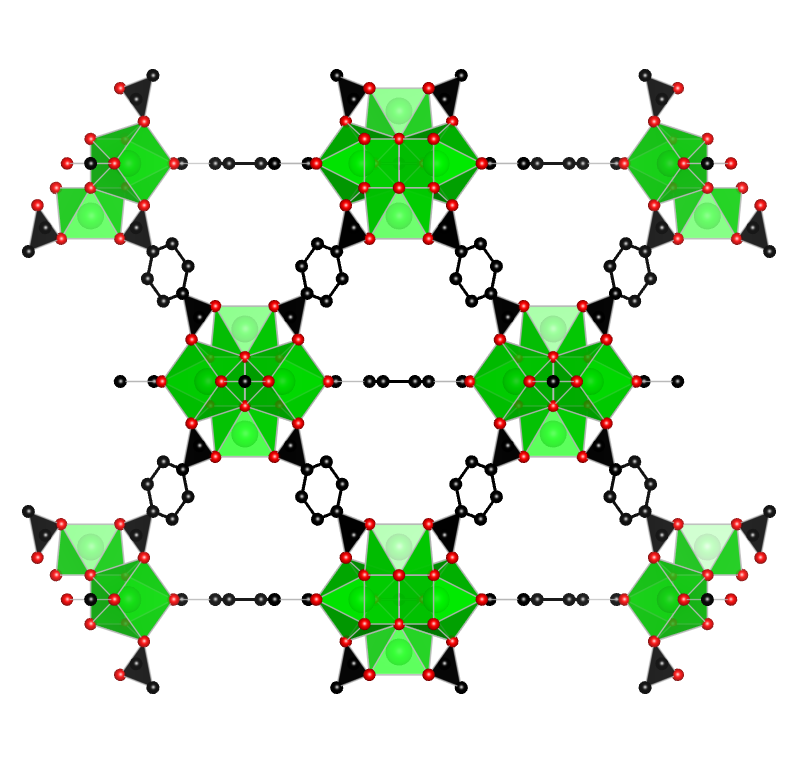
\includegraphics[width=\textwidth]{tga/uio66}%
        }%
    \end{subfigure}

    \begin{subfigure}{0.6\textwidth}
        \parbox[c]{0.1\linewidth}{\caption{}\label{fig:shaping:tgamil100}}%
        \parbox[b]{0.7\linewidth}{%
        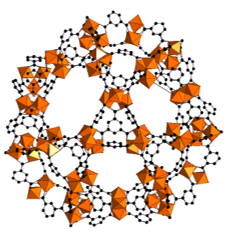
\includegraphics[width=\textwidth]{tga/mil100}%
        }%
    \end{subfigure}

    \begin{subfigure}{0.6\textwidth}
        \parbox[c]{0.1\linewidth}{\caption{}\label{fig:shaping:tgamil127}}%
        \parbox[b]{0.7\linewidth}{%
        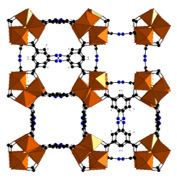
\includegraphics[width=\textwidth]{tga/mil127}%
        }%
    \end{subfigure}
    
    \caption{High resolution TGA curves recoded under argon 
    on (a) UiO-66(Zr), (b) MIL-100(Fe) and (c) MIL-127(Fe). The 
    original powders are depicted in red and the shaped material
    in blue.}%
    \label{fig:shaping:tgacurves}

\end{figure}
